%%%%%%%%%%%%%%%%%%%%%%%%%%%%%%%%%%%%%%%%%
% Beamer Presentation
% LaTeX Template
% Version 1.0 (10/11/12)
%
% This template has been downloaded from:
% http://www.LaTeXTemplates.com
%
% License:
% CC BY-NC-SA 3.0 (http://creativecommons.org/licenses/by-nc-sa/3.0/)
%
%%%%%%%%%%%%%%%%%%%%%%%%%%%%%%%%%%%%%%%%%

%----------------------------------------------------------------------------------------
%	PACKAGES AND THEMES
%----------------------------------------------------------------------------------------

\documentclass{beamer}

\mode<presentation> {

% The Beamer class comes with a number of default slide themes
% which change the colors and layouts of slides. Below this is a list
% of all the themes, uncomment each in turn to see what they look like.

%\usetheme{default}
%\usetheme{AnnArbor}
%\usetheme{Antibes}
%\usetheme{Bergen}
%\usetheme{Berkeley}
%\usetheme{Berlin}
%\usetheme{Boadilla}
%\usetheme{CambridgeUS}
%\usetheme{Copenhagen}
%\usetheme{Darmstadt}
%\usetheme{Dresden}
%\usetheme{Frankfurt}
%\usetheme{Goettingen}
%\usetheme{Hannover}
%\usetheme{Ilmenau}
%\usetheme{JuanLesPins}
%\usetheme{Luebeck}
\usetheme{Madrid}
%\usetheme{Malmoe}
%\usetheme{Marburg}
%\usetheme{Montpellier}
%\usetheme{PaloAlto}
%\usetheme{Pittsburgh}
%\usetheme{Rochester}
%\usetheme{Singapore}
%\usetheme{Szeged}
%\usetheme{Warsaw}

% As well as themes, the Beamer class has a number of color themes
% for any slide theme. Uncomment each of these in turn to see how it
% changes the colors of your current slide theme.

%\usecolortheme{albatross}
%\usecolortheme{beaver}
%\usecolortheme{beetle}
%\usecolortheme{crane}
%\usecolortheme{dolphin}
%\usecolortheme{dove}
%\usecolortheme{fly}
%\usecolortheme{lily}
%\usecolortheme{orchid}
%\usecolortheme{rose}
%\usecolortheme{seagull}
%\usecolortheme{seahorse}
%\usecolortheme{whale}
%\usecolortheme{wolverine}

%\setbeamertemplate{footline} % To remove the footer line in all slides uncomment this line
%\setbeamertemplate{footline}[page number] % To replace the footer line in all slides with a simple slide count uncomment this line

%\setbeamertemplate{navigation symbols}{} % To remove the navigation symbols from the bottom of all slides uncomment this line
}

%\usepackage{graphicx} % Allows including images
\usepackage{booktabs} % Allows the use of \toprule, \midrule and \bottomrule in tables
\usepackage{subcaption}

%----------------------------------------------------------------------------------------
%	TITLE PAGE
%----------------------------------------------------------------------------------------

\title[TP3]{Trabajo Práctico III - Reconstrucción de Imágenes } % The short title appears at the bottom of every slide, the full title is only on the title page

\author[Carreira-Torres-Martino-Nahmod]{Maximiliano Martino, Edén Torres, Tobias Agustín Carreira Munich, Santiago Nahmod} % Your name
\institute[FCEyN] % Your institution as it will appear on the bottom of every slide, may be shorthand to save space
{
Facultad de Ciencias Exactas y Naturales, UBA \\ % Your institution for the title page
\medskip
}
\date{\today} % Date, can be changed to a custom date

\makeatletter
\let\@@magyar@captionfix\relax
\makeatother
\begin{document}

\begin{frame}
\titlepage % Print the title page as the first slide
\end{frame}

\begin{frame}
\frametitle{Overview} % Table of contents slide, comment this block out to remove it
\tableofcontents % Throughout your presentation, if you choose to use \section{} and \subsection{} commands, these will automatically be printed on this slide as an overview of your presentation
\end{frame}

%----------------------------------------------------------------------------------------
%	PRESENTATION SLIDES
%----------------------------------------------------------------------------------------

%------------------------------------------------
\section{Introducción} % Sections can be created in order to organize your presentation into discrete blocks, all sections and subsections are automatically printed in the table of contents as an overview of the talk
%------------------------------------------------

\begin{frame}
\frametitle{Introducción}
% TODO: intro - CORTO (Todos ya saben esto)
%       Introduccion al problema y muy general la solucion.
Objetivos:
\begin{itemize}
	\item Estudiar la aplicación de técnicas algorítmicas y de aproximación para la reconstrucción de imágenes tomográficas computadas.
	\item Evaluar nuestro modelo de reconstrucción mediante la simulación de un tomógrafo.
	\item Resolver los errores de medición de los instrumentos utilizados.
\end{itemize}
    \begin{figure}
      \centering
      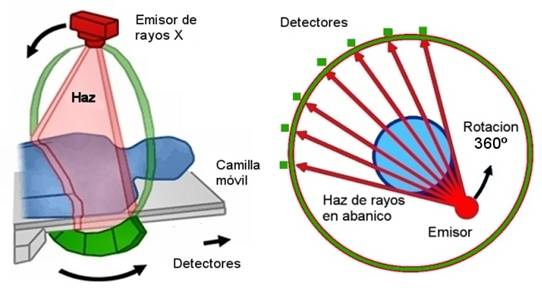
\includegraphics[height=0.35\textheight]{imagenes/tomografo.png}
	\caption{Imagen de un fotografo real}
\footnote{\url{www.geocities.ws/cytparatodos/vidaytierra/tomografia/index.htm}}
    \end{figure}
 
 
\end{frame}

%------------------------------------------------
\section{Base Teórica}
%------------------------------------------------

\begin{frame}
\frametitle{Base Teórica}
% TODO: Base Teorica - CORTO (Todos ya saben esto)
%       La justificacion de usar SVD y nada mas.

Utilización de CML:
\begin{itemize}
	\item El sistema estará sobre-determinado y los instrumentos poseen errores de medición, por lo cual no hallaremos una solución exacta a nuestro problema
	\item Debemos utilizar métodos de aproximación, en particular Cuadrados Mínimos Lineales
\end{itemize}
Utilización de SVD:
\begin{itemize}
	\item Utilizar ecuaciones normales para la resolución de CML presenta el problema de elevar al cuadrado el número de condición de la matriz
	\item La descomposición SVD nos asegura la estabilidad númerica 
\end{itemize}

\end{frame}


\begin{frame}
\frametitle{Base Teórica}

	\textbf{Aproximación de menor rango}

	Al calcular SVD de una matriz $D$, si nos detenemos luego de calcular $k < rg(D)$ valores singulares de la matriz,
	estamos consiguiendo la matriz de rango k que minimiza la distancia \textit{Frobenius} a $D$.

\end{frame}

%------------------------------------------------
\section{Desarrollo}
%------------------------------------------------
\subsection{Decisiones de diseño}
%------------------------------------------------

\begin{frame}
\frametitle{Desarrollo}
\framesubtitle{Decisiones de diseño}
% TODO: Deciciones de diseño
%       Aca solo hay que mencionar caracteristicas que nos diferencien de otros grupos. Ej: Como guardamos las matrices, como elegimos el ruido, el uso de threads y otras cosas locas, como guardamos los resultados.
Diseño:
\begin{itemize}
	\item La imagen representada como una matriz de int
	\item Modelamos los rayos con dos puntos (origen/destino)
	\item Simulación de ruido utilizando una distribucion normal
	\item Saturamos aquellos datos fuera del rango posible para un píxel (0-255)
	\item Utilización del Método de la Potencia con deflación para el cálculo de autovalores realizando 100 iteraciones
\end{itemize}

\end{frame}

%------------------------------------------------
\subsection{Decisiones de optimización}
%------------------------------------------------

\begin{frame}
\frametitle{Desarrollo}
\framesubtitle{Decisiones de optimización}

Optimizaciones:
\begin{itemize}
	\item Reutilización de SVD
	\item Paralelización de calculos utilizando threads (Tanto el cálculo de $D^{t}D$ como el Método de la Potencia usan repetidas veces la multiplicación entre matriz y vector)
\end{itemize}


\end{frame}

%------------------------------------------------
\section{Experimentación}
%------------------------------------------------

\begin{frame}
\frametitle{Experimentación}
\textbf{\underline{Imágenes Base}}
\begin{figure}[H]
	\centering
  \begin{subfigure}[t]{0.3\textwidth}
      \centering
      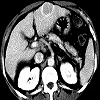
\includegraphics[height=1.0in]{imagenes/tomo.png}
      \caption{Tomografía 1}
  \end{subfigure}
  ~ 
  \begin{subfigure}[t]{0.3\textwidth}
      \centering
      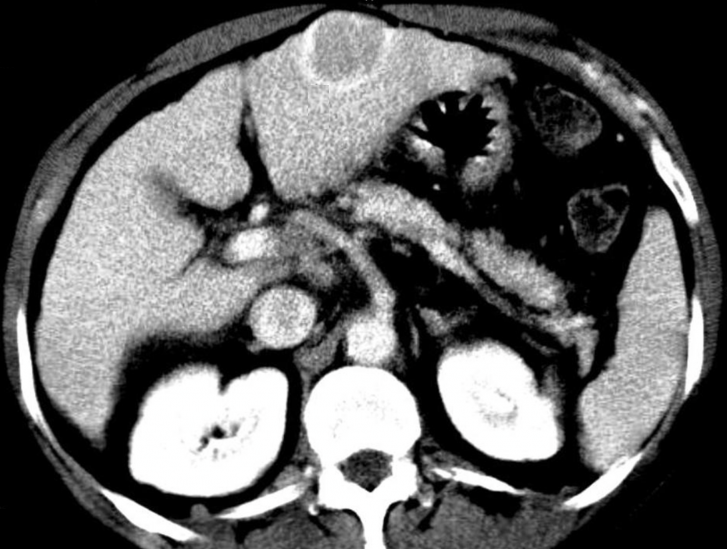
\includegraphics[height=1.0in]{imagenes/tomo2.png}
      \caption{Tomografía 2}
  \end{subfigure}
  ~ 
  \begin{subfigure}[t]{0.3\textwidth}
      \centering
      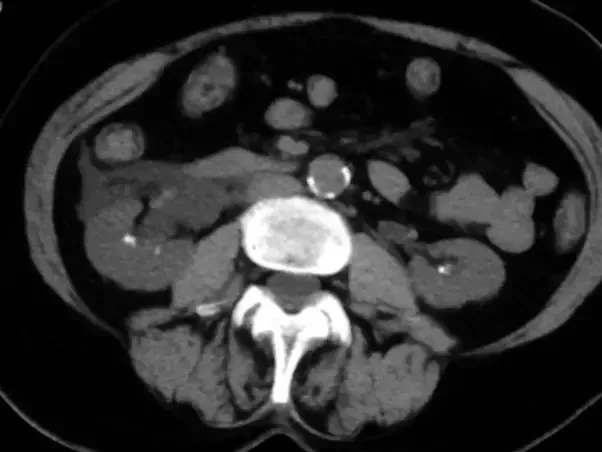
\includegraphics[height=1.0in]{imagenes/tomo3.png}
      \caption{Tomografía 3}
  \end{subfigure}
\end{figure}
\end{frame}

%------------------------------------------------
\subsection{Elección de rayos}
%------------------------------------------------

\begin{frame}
\frametitle{Experimentación}
\framesubtitle{Elección de rayos}
\textbf{\underline{Rayos Aleatorios}}
  \begin{figure}
    \centering
    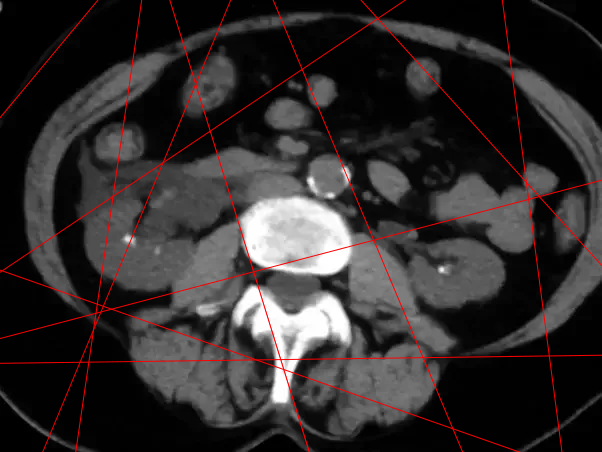
\includegraphics[height=0.75\textheight]{imagenes/random.png}
  \end{figure}
\end{frame}

%------------------------------------------------

\begin{frame}
  \frametitle{Experimentación}
  \framesubtitle{Elección de rayos}
	\textbf{\underline{Rayos Rotados}} \only<2>{¿Algún problema?}
    \begin{figure}
      \centering
      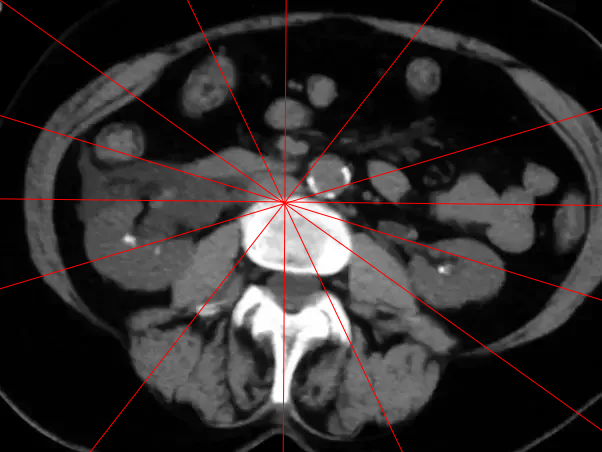
\includegraphics[height=0.75\textheight]{imagenes/rotados.png}
    \end{figure}
\end{frame}

%------------------------------------------------

\begin{frame}
  \frametitle{Experimentación}
  \framesubtitle{Elección de rayos}
  \textbf{\underline{Rayos Laterales}}
    \begin{figure}
      \centering
      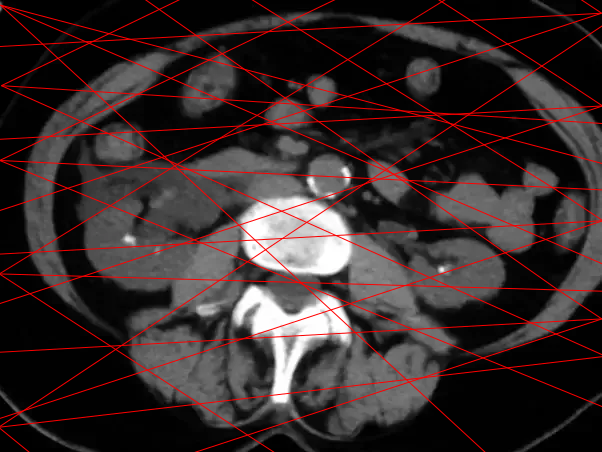
\includegraphics[height=0.75\textheight]{imagenes/lateral.png}
    \end{figure}
\end{frame}

%------------------------------------------------

\begin{frame}
  \frametitle{Experimentación}
  \framesubtitle{Elección de rayos}
  \textbf{\underline{Rayos de todos los bordes}}
    \begin{figure}
      \centering
      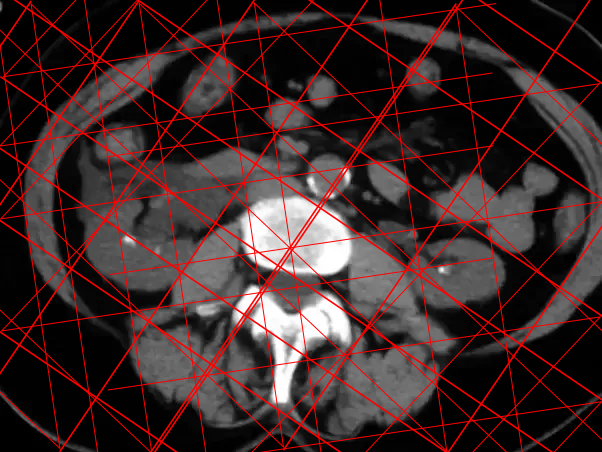
\includegraphics[height=0.75\textheight]{imagenes/allborders.png}
    \end{figure}
\end{frame}

%------------------------------------------------
\subsection{Métricas}
%------------------------------------------------

\begin{frame}
\frametitle{Experimentación}
\framesubtitle{Métricas}
\begin{block}{PSNR}
  \begin{equation*}
    PSNR = 10 \times \log_{10}(\frac{MAX^2_{u}}{ECM})
 \end{equation*}
 
 Donde $MAX^2_{u}$ define el rango máximo de la imagen y ECM es el error cuadrático medio donde se compara la imagen ideal a la imagen reconstruida.
\end{block}
\end{frame}

%------------------------------------------------
\subsection{Nivel de ruido y discretización}
%------------------------------------------------

\begin{frame}
\frametitle{Experimentación}
\framesubtitle{Nivel de ruido y discretización}
\underline{PSNR Vs. ruido para distintos tamaños de discretización de Tomografía 1}
\begin{figure}[H]
  \centering
  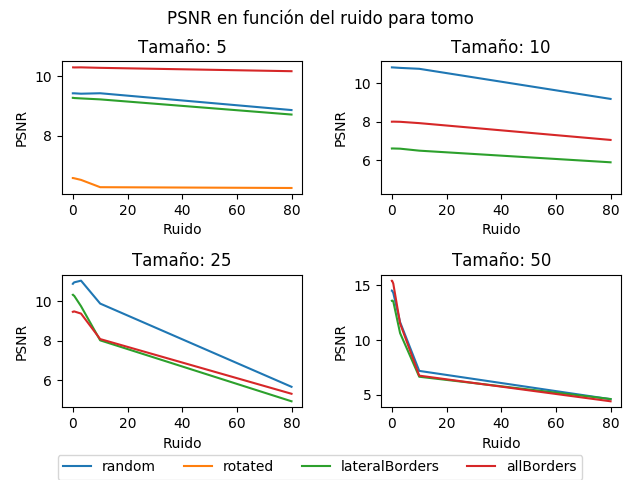
\includegraphics[height=0.75\textheight]{../graficos/noise/tomo/noise_graph.png}
\end{figure}
\end{frame}

%------------------------------------------------

\begin{frame}
  \frametitle{Experimentación}
  \framesubtitle{Nivel de ruido y discretización}
  \underline{PSNR Vs. ruido para distintos tamaños de discretización de Tomografía 3}
  \begin{figure}[H]
    \centering
    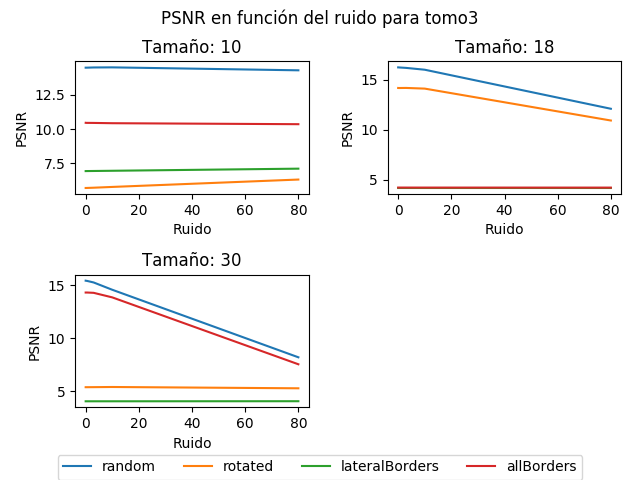
\includegraphics[height=0.75\textheight]{../graficos/noise/tomo3/noise_graph.png}
  \end{figure}
\end{frame}

%------------------------------------------------

\begin{frame}
  \frametitle{Experimentación}
  \framesubtitle{Nivel de ruido y discretización}
  \underline{Tomografía 1 con el método random con ruido 0.1}
  \begin{figure}[H]
    \centering
      \begin{subfigure}[t]{0.3\textwidth}
          \centering
          
\includegraphics[height=1.0in]{imagenes/noise/1.png}
          \caption{Tomografía size 10}
      \end{subfigure}
      ~ 
      \begin{subfigure}[t]{0.3\textwidth}
          \centering
          
\includegraphics[height=1.0in]{imagenes/noise/2.png}
          \caption{Tomografía size 25}
      \end{subfigure}
      ~ 
      \begin{subfigure}[t]{0.3\textwidth}
          \centering
          
\includegraphics[height=1.0in]{imagenes/noise/3.png}
          \caption{Tomografía size 50}
      \end{subfigure}
  \end{figure}
\end{frame}

%------------------------------------------------

\begin{frame}
  \frametitle{Experimentación}
  \framesubtitle{Nivel de ruido y discretización}
  \underline{Tomografía 1 con el método allBorders con ruido 0.1}
  \begin{figure}[H]
    \centering
      \begin{subfigure}[t]{0.3\textwidth}
          \centering
          
\includegraphics[height=1.0in]{imagenes/noise/4.png}
          \caption{Tomografía size 10}
      \end{subfigure}
      ~ 
      \begin{subfigure}[t]{0.3\textwidth}
          \centering
          
\includegraphics[height=1.0in]{imagenes/noise/5.png}
          \caption{Tomografía size 25}
      \end{subfigure}
      ~ 
      \begin{subfigure}[t]{0.3\textwidth}
          \centering
          
\includegraphics[height=1.0in]{imagenes/noise/6.png}
          \caption{Tomografía size 50}
      \end{subfigure}
  \end{figure}
\end{frame}

%------------------------------------------------

\begin{frame}
  \frametitle{Experimentación}
  \framesubtitle{Nivel de ruido y discretización}
  \begin{figure}[H]
    \centering
    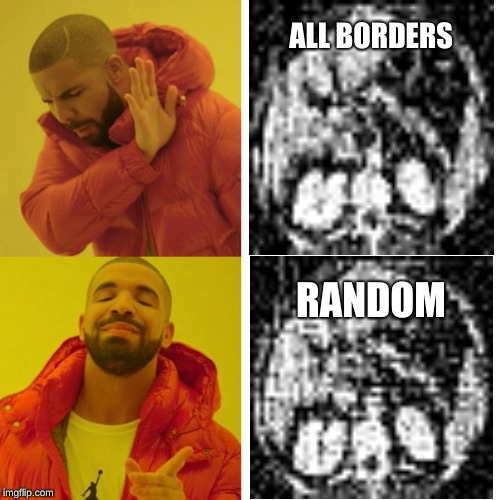
\includegraphics[height=0.75\textheight]{imagenes/meme.jpg}
  \end{figure}
\end{frame}

%------------------------------------------------
\subsection{Cantidad de rayos y discretización}
%------------------------------------------------

\begin{frame}
\frametitle{Experimentación}
\framesubtitle{Cantidad de rayos y discretización}
\underline{PSNR Vs. rayos/pixeles para distintos tamaños de Tomografía 1}
\begin{figure}[H]
  \centering
  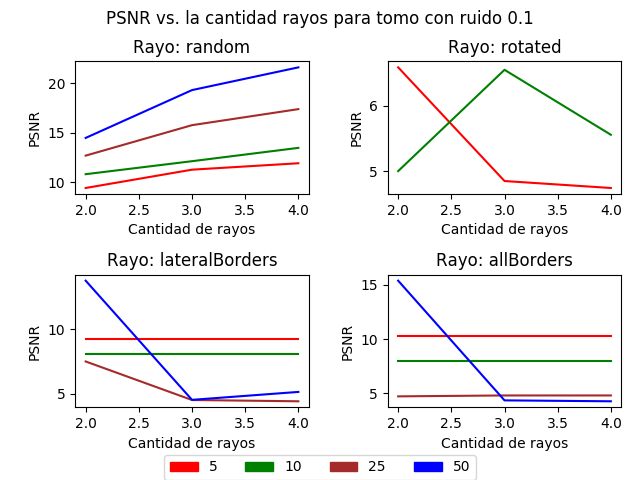
\includegraphics[height=0.75\textheight]{../graficos/ray_params/tomo/noise_graph_0.png}
\end{figure}
\end{frame}

%------------------------------------------------

\begin{frame}
  \frametitle{Experimentación}
  \framesubtitle{Cantidad de rayos y discretización}
  \underline{PSNR Vs. rayos/pixeles para distintos tamaños de Tomografía 3}
  \begin{figure}[H]
    \centering
    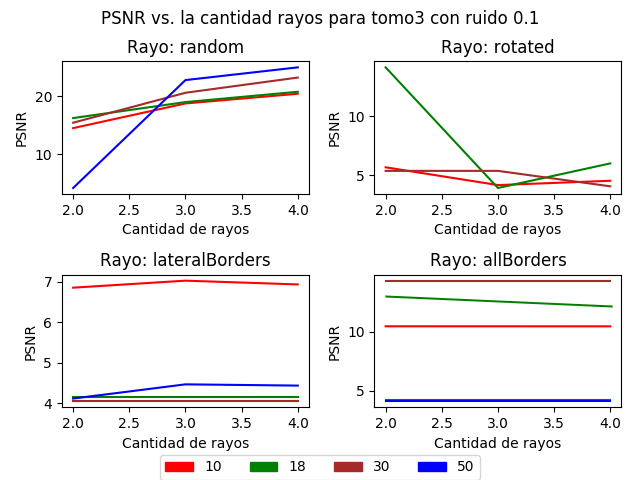
\includegraphics[height=0.75\textheight]{../graficos/ray_params/tomo3/noise_graph_0.png}
  \end{figure}
\end{frame}

%------------------------------------------------

\begin{frame}
  \frametitle{Experimentación}
  \framesubtitle{Cantidad de rayos y discretización}
  \underline{Tomografía 1 - Random - Ruido 0.1 - Size 50, variando la cantida de rayos}
  \begin{figure}[H]
    \centering
      \begin{subfigure}[t]{0.3\textwidth}
          \centering
          
\includegraphics[height=1.0in]{imagenes/ray_n/1.png}
          \caption{Tomografía 150\% del size de rayos}
      \end{subfigure}
      ~ 
      \begin{subfigure}[t]{0.3\textwidth}
          \centering
          
\includegraphics[height=1.0in]{imagenes/ray_n/2.png}
          \caption{Tomografía 200\% del size de rayos}
      \end{subfigure}
      ~ 
      \begin{subfigure}[t]{0.3\textwidth}
          \centering
          
\includegraphics[height=1.0in]{imagenes/ray_n/3.png}
          \caption{Tomografía 300\% del size de rayos}
      \end{subfigure}
      \\
      \begin{subfigure}[t]{0.3\textwidth}
          \centering
          
\includegraphics[height=1.0in]{imagenes/ray_n/4.png}
          \caption{Tomografía 400 \% del size de  rayos}
      \end{subfigure}
      ~ 
      \begin{subfigure}[t]{0.3\textwidth}
          \centering
          
\includegraphics[height=1.0in]{imagenes/ray_n/5.png}
          \caption{Tomografía 500 \% del size de rayos}
      \end{subfigure}
  \end{figure}
\end{frame}

%------------------------------------------------
\subsection{Cantidad de valores singulares}
%------------------------------------------------

\begin{frame}
\frametitle{Experimentación}
\framesubtitle{Cantidad de valores singulares}
\underline{PSNR Vs. porcentaje de autovalores que calculamos para Tomografía 1}
\begin{figure}[H]
  \centering
  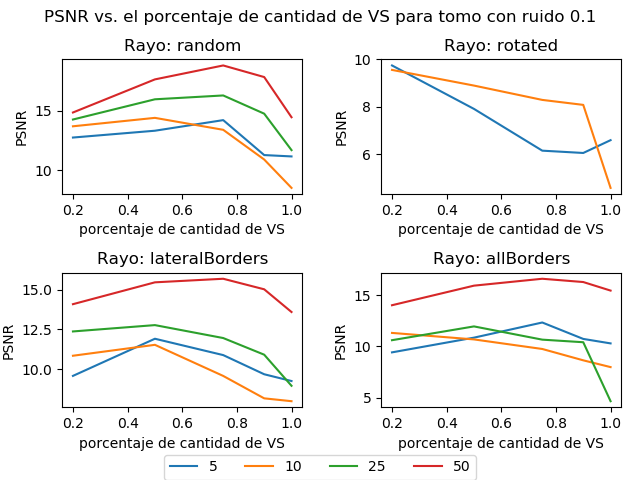
\includegraphics[height=0.75\textheight]{../graficos/eigens/tomo/noise_graph_2.png}
\end{figure}
\end{frame}

%------------------------------------------------
\subsection{Tiempo de valores singulares}
%------------------------------------------------

\begin{frame}
  \frametitle{Experimentación}
  \framesubtitle{Tiempo de valores singulares}
  \textbf{\underline{Rewind}}
  \begin{itemize}
    \item<1-> Método de la Potencia con 100 iteraciones.
    \item<2-> Calcular cada autovalor tiene un costo de $O(n^2 * 100)$
  \end{itemize}
\end{frame}

%------------------------------------------------

\begin{frame}
  \frametitle{Experimentación}
  \framesubtitle{Tiempo de valores singulares}
  \underline{Tiempo de cálculo de CML Vs. del porcentaje de valores singulares}
  \begin{figure}[H]
    \centering
    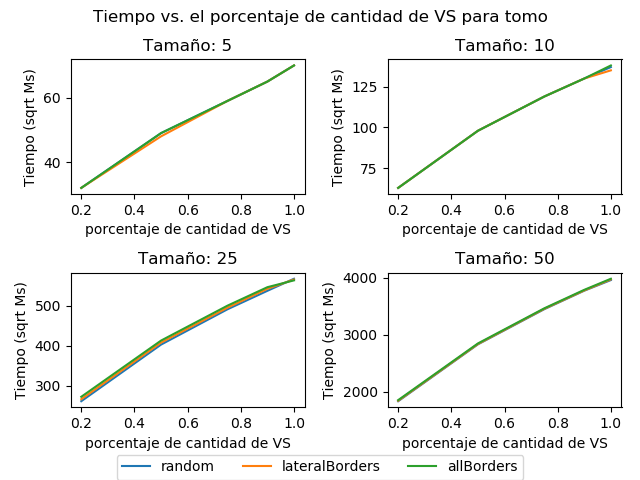
\includegraphics[height=0.75\textheight]{../graficos/eigens-time/tomo/noise_graph.png}
  \end{figure}
\end{frame}

%------------------------------------------------
\subsection{Tamaño de la imagen de salida}
%------------------------------------------------

\begin{frame}
\frametitle{Experimentación}
\framesubtitle{Tamaño de la imagen de salida}
\underline{PSNR Vs. el tamaño de la imagen de salida para Tomografía 1}
\begin{figure}[H]
  \centering
  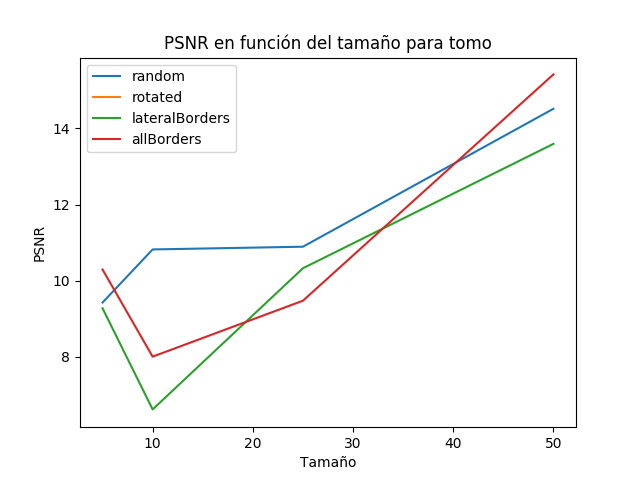
\includegraphics[height=0.75\textheight]{../graficos/size/tomo/noise_graph.png}
\end{figure}
\end{frame}

%------------------------------------------------
\section{Conclusiones}
%------------------------------------------------

\begin{frame}
\frametitle{Conclusiones}
% TODO: Concluciones 
%       Short and to the point.
Pros:
\begin{itemize}
	\item Gran potencial en el método para este tipo de problemas.
	\item No observamos diferencias al probar con distintas imágenes.
	\item El mejor método para generar rayos fue el random .
	\item Aumentar las cantidad de rayos y de valores singulares que calculamos
		no mejora siempre la calidad.
\end{itemize}

Cons:
\begin{itemize}
	\item El método tiene problemas de estabilidad numérica si no se usa SVD.
	\item Discretizar la imagen con valores grandes aumenta mucho los tiempos.
\end{itemize}
\end{frame}

%------------------------------------------------

\begin{frame}
  \Huge{\centerline{Fin}}
\end{frame}
%------------------------------------------------
%------------------------------------------------
%------------------------------------------------
%------------------------------------------------

\end{document}
